
\section{Data Definitions and Training Distributions}\label{app:data-characteristics}
Taxi events are pickup counts in active spatial-cell hours; Intermittent
events are positive site--part order quantities; RAF events are positive
monthly spare-parts demands. Instacart events aggregate product rows for a
user on the same recorded activity day. Its quantity is a basket-size proxy,
not a count of physical units. In these event sequences, empty calendar
periods contribute to the recorded gap rather than separate zero-quantity
targets. Gaps retain their dataset-specific units (Table~\ref{tab:train-characteristics}).

We describe each frozen training population using the same definitions.
Quantity quantiles include all train event rows. Gap and usable-history
statistics describe the canonical prediction targets, which exclude the
first event of each series. For a target, usable history is the number of
observed predecessor events retained by the dataset's recorded-time window
and sequence-length cap. It excludes the target and padding. Thus it differs
from both elapsed calendar time and the total number of events in a series.
Train quantities and histories characterize available learning evidence;
the validation counts in Appendix~\ref{app:strata} describe a different
population later in each sequence.

For adjacent quantities, let $x_{e,j}=\log(1+q_{e,j-1})$ and
$y_{e,j}=\log(1+q_{e,j})$ for train pairs in series $e$. We compute
\begin{equation}
 r_{\mathrm{within}}=\operatorname{Corr}
 \bigl(x_{e,j}-\bar x_e,\;y_{e,j}-\bar y_e\bigr),
 \label{eq:within-correlation}
\end{equation}
pooling the centered pairs across series. The two means are computed
separately over each series' predecessor and successor members. This
pair-weighted statistic removes differences in average scale between series;
it is not an average of series-specific correlation coefficients.

\begin{table}[t]
\caption{Train-only event characteristics. Quantity summaries use all train event rows; gap, usable-history, and adjacent-pair summaries use train targets after excluding each series\textquotesingle{} first event. Quantiles use the nearest observed value. Instacart gaps are top-coded at 30 days.}
\label{tab:train-characteristics}\centering\scriptsize
\setlength{\tabcolsep}{4pt}
\begin{tabular}{lrrrr}
\toprule
Characteristic & Taxi & Intermittent & RAF & Instacart\\
\midrule
Time unit & Hour & Week & Month & Day\\
Train series & 131 & 5,000 & 5,000 & 206,209\\
Train event rows & 38,524 & 398,824 & 30,779 & 2,197,401\\
Train targets & 38,393 & 393,824 & 25,779 & 1,991,192\\
Quantity: median & 7 & 2 & 2 & 8\\
Quantity: 95th percentile & 1,562 & 46 & 60 & 25\\
Quantity: 99th percentile & 3,449 & 187 & 200 & 35\\
Quantity: maximum & 6,322 & 477 & 2,062 & 175\\
Recorded gap: median & 1 & 3 & 6 & 7\\
Recorded gap: 95th percentile & 5 & 5 & 23 & 30\\
Usable history: median & 129 & 40 & 3 & 5\\
Usable history: 95th percentile & 168 & 144 & 8 & 14\\
History $\le7$ events (\%) & 2.41 & 8.89 & 93.58 & 72.13\\
Within-series log correlation & 0.749 & 0.928 & -0.105 & 0.037\\
Equal adjacent quantities (\%) & 20.33 & 61.99 & 33.30 & 10.24\\
\bottomrule
\end{tabular}
\end{table}

\begin{figure}[t]
\centering
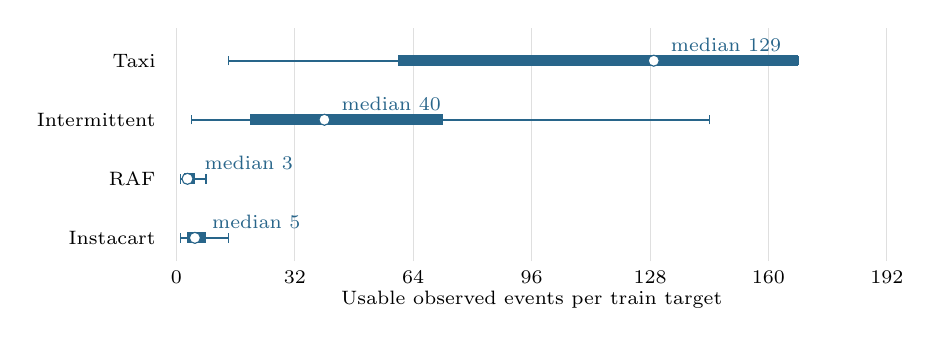
\begin{tikzpicture}[x=.047cm,y=.75cm,font=\scriptsize]
\definecolor{plotblue}{RGB}{40,101,138}
\draw[gray!25] (0,-.4)--(0,3.55);
\node[below] at (0,-.4) {0};
\draw[gray!25] (32,-.4)--(32,3.55);
\node[below] at (32,-.4) {32};
\draw[gray!25] (64,-.4)--(64,3.55);
\node[below] at (64,-.4) {64};
\draw[gray!25] (96,-.4)--(96,3.55);
\node[below] at (96,-.4) {96};
\draw[gray!25] (128,-.4)--(128,3.55);
\node[below] at (128,-.4) {128};
\draw[gray!25] (160,-.4)--(160,3.55);
\node[below] at (160,-.4) {160};
\draw[gray!25] (192,-.4)--(192,3.55);
\node[below] at (192,-.4) {192};
\node[anchor=east] at (-3,3) {Taxi};
\draw[plotblue,line width=.6pt] (14.0,3)--(168.0,3);
\draw[plotblue,line width=4pt] (60.0,3)--(168.0,3);
\draw[plotblue] (14.0,2.92)--(14.0,3.08) (168.0,2.92)--(168.0,3.08);
\filldraw[draw=plotblue,fill=white] (129.0,3) circle[radius=2pt];
\node[anchor=west,text=plotblue] at (131.0,3.27) {median 129};
\node[anchor=east] at (-3,2) {Intermittent};
\draw[plotblue,line width=.6pt] (4.0,2)--(144.0,2);
\draw[plotblue,line width=4pt] (20.0,2)--(72.0,2);
\draw[plotblue] (4.0,1.92)--(4.0,2.08) (144.0,1.92)--(144.0,2.08);
\filldraw[draw=plotblue,fill=white] (40.0,2) circle[radius=2pt];
\node[anchor=west,text=plotblue] at (42.0,2.27) {median 40};
\node[anchor=east] at (-3,1) {RAF};
\draw[plotblue,line width=.6pt] (1.0,1)--(8.0,1);
\draw[plotblue,line width=4pt] (2.0,1)--(5.0,1);
\draw[plotblue] (1.0,0.92)--(1.0,1.08) (8.0,0.92)--(8.0,1.08);
\filldraw[draw=plotblue,fill=white] (3.0,1) circle[radius=2pt];
\node[anchor=west,text=plotblue] at (5.0,1.27) {median 3};
\node[anchor=east] at (-3,0) {Instacart};
\draw[plotblue,line width=.6pt] (1.0,0)--(14.0,0);
\draw[plotblue,line width=4pt] (3.0,0)--(8.0,0);
\draw[plotblue] (1.0,-0.08)--(1.0,0.08) (14.0,-0.08)--(14.0,0.08);
\filldraw[draw=plotblue,fill=white] (5.0,0) circle[radius=2pt];
\node[anchor=west,text=plotblue] at (7.0,0.27) {median 5};
\node at (96,-1.05) {Usable observed events per train target};
\end{tikzpicture}
\caption{Train-history distributions under the frozen input windows. Thin lines span the 5th--95th percentiles, thick lines the 25th--75th percentiles, and circles mark medians. These are event-weighted train summaries, not validation performance curves.}
\label{fig:train-history}
\end{figure}

Taxi and Intermittent retain substantially longer histories and stronger
within-series adjacent association than the other datasets.
RAF's median usable train history is three events, and 93.58\% of targets
have at most seven; the corresponding Instacart values are five and 72.13\%.
RAF's centered correlation is $-0.105$, compared with Instacart's $0.037$.
The RAF estimate summarizes very short sequences after mean removal, so it
should not be read as a stable negative dependence law. These distributions
make history correction's dataset dependence plausible, while the observed
error comparisons below establish where its gains and losses occur.

\section{Validation Errors by Quantity and Usable History}\label{app:strata}
\subsection{Partitions and Aggregation}
The analysis uses the completed selected-checkpoint validation records for
all seven models in Table~\ref{tab:main}: four datasets and three seeds,
84 runs in total. Every stratum uses the same earliest minimum-RMSE
checkpoint as the overall results. The tables focus on TitanTPP and the
external model with the lowest overall mean validation RMSE on each dataset:
RMTPP on Taxi and Intermittent, and S2P2 on RAF and Instacart. This comparator
is held fixed across strata, including strata where another model performs
better.

Quantity boundaries are the frozen train-derived 50th, 90th, 95th, and
99th percentiles: $(7,686,1562,3449)$ for Taxi, $(2,31,46,187)$ for
Intermittent, $(2,30,60,200)$ for RAF, and $(8,20,25,35)$ for Instacart.
Upper boundaries belong to the lower bin. History boundaries reuse the
stored partitions: $(64,128)$ observed events for Taxi, Intermittent, and
RAF, and $(1,3,7,15,31)$ for Instacart. The finer Instacart partition
resolves its shorter histories. These dataset-specific bins support
within-dataset diagnosis; they are not identical history-length groups
across all four datasets. RAF's validation targets all fall in the first
stored history bin, so that partition cannot resolve its short-history
differences. We retain the empty cells in Table~\ref{tab:strata-history}.

Within each seed, MAE averages absolute error over targets and RMSE is the
square root of mean squared error. Tables~\ref{tab:strata-quantity}
and~\ref{tab:strata-history} report arithmetic means of those metrics over
seeds 42, 52, and 62. Each $N$ counts targets once per seed, not three times;
the target populations are identical across models and seeds. Duration NLL
in the overall comparison also uses the same selected checkpoints.

\begin{table}[p]
\caption{Quantity-stratum validation errors at the selected checkpoints. Entries are arithmetic means over seeds 42, 52, and 62; $N$ is the number of targets per seed. The external comparator is fixed per dataset by the overall RMSE in Table~\ref{tab:main}, not selected within each bin. Empty strata have no estimated error.}
\label{tab:strata-quantity}\centering\scriptsize
\setlength{\tabcolsep}{4pt}
\begin{tabular}{lrrrrr}
\toprule
Stratum & $N$ & \multicolumn{2}{c}{TitanTPP} & \multicolumn{2}{c}{External comparator}\\
 & & MAE & RMSE & MAE & RMSE\\
\midrule
\multicolumn{6}{l}{\textit{Taxi vs. RMTPP}}\\
$q\le 7$ & 4,364 & 2.3003 & 9.8889 & 2.1501 & 7.3292\\
$7<q\le 686$ & 3,138 & 23.4775 & 50.8082 & 21.9881 & 46.0420\\
$686<q\le 1562$ & 386 & 114.2264 & 160.7697 & 139.5607 & 201.5555\\
$1562<q\le 3449$ & 301 & 197.8383 & 271.7508 & 242.0791 & 320.5319\\
$q> 3449$ & 79 & 310.1894 & 384.9824 & 387.6200 & 509.8502\\
\addlinespace
\multicolumn{6}{l}{\textit{Intermittent vs. RMTPP}}\\
$q\le 2$ & 45,036 & 0.1487 & 0.2621 & 0.0731 & 0.1535\\
$2<q\le 31$ & 29,579 & 0.8965 & 1.4835 & 1.0205 & 1.4419\\
$31<q\le 46$ & 7,124 & 1.4464 & 2.2055 & 1.7433 & 2.4149\\
$46<q\le 187$ & 3,405 & 2.9671 & 4.2619 & 5.2337 & 6.6144\\
$q> 187$ & 1,141 & 5.9795 & 8.1891 & 11.8304 & 16.3628\\
\addlinespace
\multicolumn{6}{l}{\textit{RAF vs. S2P2}}\\
$q\le 2$ & 3,626 & 1.9835 & 6.3967 & 1.9552 & 7.1732\\
$2<q\le 30$ & 2,555 & 7.4744 & 14.3371 & 7.6838 & 15.9466\\
$30<q\le 60$ & 235 & 25.5628 & 30.9633 & 28.4258 & 33.9447\\
$60<q\le 200$ & 224 & 69.3894 & 81.9318 & 65.8432 & 77.9821\\
$q> 200$ & 50 & 280.9391 & 325.8366 & 277.7154 & 324.3119\\
\addlinespace
\multicolumn{6}{l}{\textit{Instacart vs. S2P2}}\\
$q\le 8$ & 247,651 & 2.7184 & 3.8081 & 2.8722 & 4.0783\\
$8<q\le 20$ & 202,534 & 3.6871 & 4.6741 & 3.7605 & 4.8145\\
$20<q\le 25$ & 27,322 & 7.9877 & 9.0866 & 7.4211 & 8.6749\\
$25<q\le 35$ & 20,190 & 11.8469 & 13.1561 & 10.6341 & 12.2964\\
$q> 35$ & 6,036 & 22.0811 & 24.6419 & 20.5236 & 23.4686\\
\bottomrule
\end{tabular}
\end{table}

\begin{table}[p]
\caption{Usable-history-stratum validation errors at the selected checkpoints. Entries are arithmetic means over seeds 42, 52, and 62; $N$ is the number of targets per seed. The external comparator is fixed per dataset by the overall RMSE in Table~\ref{tab:main}, not selected within each bin. Empty strata have no estimated error.}
\label{tab:strata-history}\centering\scriptsize
\setlength{\tabcolsep}{4pt}
\begin{tabular}{lrrrrr}
\toprule
Stratum & $N$ & \multicolumn{2}{c}{TitanTPP} & \multicolumn{2}{c}{External comparator}\\
 & & MAE & RMSE & MAE & RMSE\\
\midrule
\multicolumn{6}{l}{\textit{Taxi vs. RMTPP}}\\
$h\le 64$ & 1,241 & 0.5174 & 0.8503 & 0.5107 & 0.8422\\
$64<h\le 128$ & 1,475 & 1.2124 & 2.5664 & 1.2119 & 2.6314\\
$h> 128$ & 5,552 & 37.7208 & 97.2636 & 42.0243 & 115.5907\\
\addlinespace
\multicolumn{6}{l}{\textit{Intermittent vs. RMTPP}}\\
$h\le 64$ & 25,088 & 0.8210 & 1.3842 & 1.0308 & 2.0659\\
$64<h\le 128$ & 28,456 & 1.1389 & 2.5081 & 1.6594 & 3.9493\\
$h> 128$ & 32,741 & 0.2272 & 0.6452 & 0.1263 & 0.5260\\
\addlinespace
\multicolumn{6}{l}{\textit{RAF vs. S2P2}}\\
$h\le 64$ & 6,690 & 9.2506 & 33.9507 & 9.2730 & 33.9947\\
$64<h\le 128$ & 0 & -- & -- & -- & --\\
$h> 128$ & 0 & -- & -- & -- & --\\
\addlinespace
\multicolumn{6}{l}{\textit{Instacart vs. S2P2}}\\
$h\le 1$ & 261 & 7.1888 & 10.6058 & 7.1550 & 10.5516\\
$1<h\le 3$ & 130,279 & 4.0556 & 6.0319 & 4.0574 & 5.9661\\
$3<h\le 7$ & 205,041 & 3.9482 & 5.7901 & 3.9612 & 5.7591\\
$7<h\le 15$ & 140,970 & 4.0272 & 5.8757 & 4.0354 & 5.8739\\
$15<h\le 31$ & 26,298 & 3.7877 & 5.7835 & 3.7780 & 5.7828\\
$h> 31$ & 884 & 4.0527 & 6.9197 & 3.8184 & 6.9017\\
\bottomrule
\end{tabular}
\end{table}

\subsection{Contributions to the Aggregate Difference}
For stratum $b$ with $N_b$ of the $N$ validation targets, define the
contribution to the MSE difference as
\begin{equation}
 C_b=\frac{1}{3N}\sum_{s\in\{42,52,62\}}
       \left(\mathrm{SSE}_{\mathrm{TitanTPP},s,b}
             -\mathrm{SSE}_{\mathrm{external},s,b}\right).
 \label{eq:mse-contribution}
\end{equation}
Then $\sum_b C_b$ equals the mean of the three seeds' overall MSE
differences. It is not the difference of squared mean RMSEs. For MAE,
the analogous contribution is $N_b/N$ times the mean within-stratum
MAE difference. Figure~\ref{fig:instacart-contributions} shows both
decompositions for Instacart.

On Taxi, the bins at or below 686 contribute $+200.886$ squared quantity
units, whereas the bins above 686 contribute $-2822.868$, yielding a net
$-2621.982$ relative to RMTPP. Intermittent has the same direction of
concentration: the bins at or below 31 contribute $+0.05969$ and those
above 31 contribute $-3.77546$. These gains are concentrated rather than
uniform: RMTPP has lower RMSE in the two lower-quantity bins of both datasets.
Their history partitions also differ. Taxi's gain is concentrated above
128 observed events, while Intermittent improves in the first two history
bins and worsens above 128. Longer history alone therefore does not order
the benefits consistently.

RAF exhibits a near cancellation against S2P2. The bins at or below 60
contribute $-31.463$ squared quantity units and those above 60 contribute
$+28.463$, leaving $-3.000$ overall. This explains why appreciable
stratum-level differences coexist with a small aggregate RMSE improvement.
The comparison is specific to S2P2; RMTPP retains the lowest overall RAF
MAE in Table~\ref{tab:main}.

For Instacart, the bins at or below 20 contribute $-1.58816$ squared
quantity units and those above 20 contribute $+1.94581$, leaving an MSE
increase of $0.35765$. The corresponding MAE difference is $-0.00712$.
Thus the low-quantity majority yields a small MAE advantage, while the
larger high-quantity errors reverse the RMSE ranking. S2P2 also has lower
mean RMSE in every nonempty stored history bin. The observed disadvantage
cannot therefore be assigned solely to a single short-history group.

\begin{figure}[t]
\centering
\begin{tikzpicture}[x=1cm,y=.52cm,font=\scriptsize]
\definecolor{plotblue}{RGB}{40,101,138}
\definecolor{plotred}{RGB}{181,85,63}
\draw[gray!25] (0.26061,-.5)--(0.26061,5.4);
\node[below] at (0.26061,-.5) {-0.08};
\draw[gray!25] (1.30303,-.5)--(1.30303,5.4);
\node[below] at (1.30303,-.5) {-0.04};
\draw[gray!25] (2.34545,-.5)--(2.34545,5.4);
\node[below] at (2.34545,-.5) {0};
\draw[gray!25] (3.38788,-.5)--(3.38788,5.4);
\node[below] at (3.38788,-.5) {0.04};
\draw[ink] (2.34545,-.4)--(2.34545,5.4);
\node[anchor=west] at (0.0,6.1) {Overall: $-0.0071$};
\node[anchor=east] at (-0.07,5) {$q\le 8$};
\fill[plotblue] (2.34545,4.73) rectangle (0.37465,5.27);
\node[anchor=east] at (-0.07,4) {$8<q\le 20$};
\fill[plotblue] (2.34545,3.73) rectangle (1.57659,4.27);
\node[anchor=east] at (-0.07,3) {$20<q\le 25$};
\fill[plotred] (2.34545,2.73) rectangle (3.14636,3.27);
\node[anchor=east] at (-0.07,2) {$25<q\le 35$};
\fill[plotred] (2.34545,1.73) rectangle (3.61229,2.27);
\node[anchor=east] at (-0.07,1) {$q> 35$};
\fill[plotred] (2.34545,0.73) rectangle (2.83182,1.27);
\node[anchor=east] at (-0.07,0) {Overall};
\fill[ink] (2.34545,-0.27) rectangle (2.15990,0.27);
\draw[gray!50] (0.0,.5)--(4.3,.5);
\node at (2.15,-1.35) {$\Delta$MAE (quantity units)};
\draw[gray!25] (6.65745,-.5)--(6.65745,5.4);
\node[below] at (6.65745,-.5) {-1};
\draw[gray!25] (7.57234,-.5)--(7.57234,5.4);
\node[below] at (7.57234,-.5) {-0.5};
\draw[gray!25] (8.48723,-.5)--(8.48723,5.4);
\node[below] at (8.48723,-.5) {0};
\draw[gray!25] (9.40213,-.5)--(9.40213,5.4);
\node[below] at (9.40213,-.5) {0.5};
\draw[gray!25] (10.31702,-.5)--(10.31702,5.4);
\node[below] at (10.31702,-.5) {1};
\draw[ink] (8.48723,-.4)--(8.48723,5.4);
\node[anchor=west] at (6.2,6.1) {Overall: $+0.3576$};
\node[anchor=east] at (6.13,5) {$q\le 8$};
\fill[plotblue] (8.48723,4.73) rectangle (6.56153,5.27);
\node[anchor=east] at (6.13,4) {$8<q\le 20$};
\fill[plotblue] (8.48723,3.73) rectangle (7.50694,4.27);
\node[anchor=east] at (6.13,3) {$20<q\le 25$};
\fill[plotred] (8.48723,2.73) rectangle (9.21105,3.27);
\node[anchor=east] at (6.13,2) {$25<q\le 35$};
\fill[plotred] (8.48723,1.73) rectangle (10.08886,2.27);
\node[anchor=east] at (6.13,1) {$q> 35$};
\fill[plotred] (8.48723,0.73) rectangle (9.72221,1.27);
\node[anchor=east] at (6.13,0) {Overall};
\fill[ink] (8.48723,-0.27) rectangle (9.14165,0.27);
\draw[gray!50] (6.2,.5)--(10.5,.5);
\node at (8.35,-1.35) {$\Delta$MSE (squared units)};
\end{tikzpicture}
\caption{Instacart quantity-stratum contributions to the overall error difference, TitanTPP minus S2P2. Each bar includes its stratum\textquotesingle{}s target share; negative values favor TitanTPP. The five bars sum to the overall difference in each panel. The panels have different units and horizontal scales.}
\label{fig:instacart-contributions}
\end{figure}
